\begin{table}
  \label{tab:creator-study}
  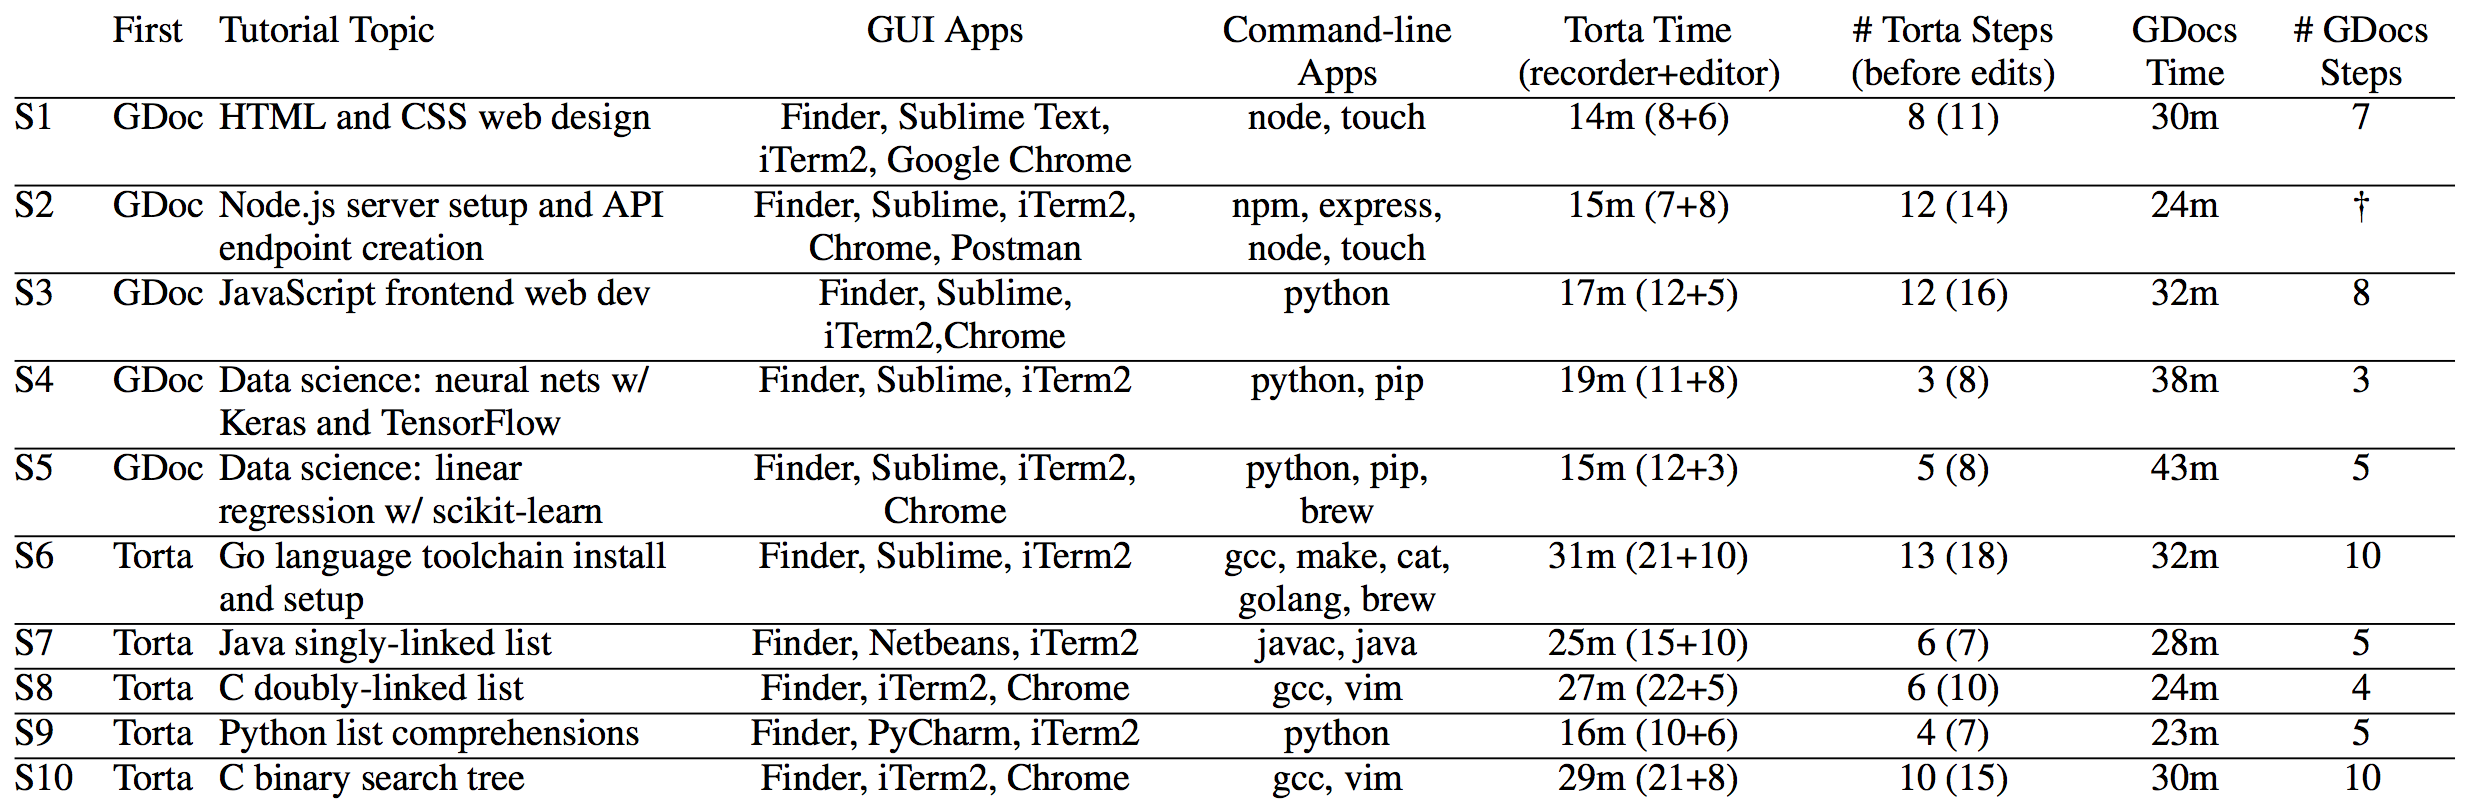
\includegraphics[width=\linewidth]{figures/torta/tbl_eval.png}
  \caption{Tutorial creator study results, showing subject IDs, which tool they used first, summary of their tutorial, time in each tool, and the numbers of steps in Torta and GDoc tutorials ($\dagger$ did not explicitly denote steps in GDocs). All times reported in minutes, with Torta split into recorder+editor times.}
\end{table}

\section{\rev{Exploratory User Studies}}

\rev{As a first pass at illustrating Torta's capabilities, we compared
users' experiences} of both creating and consuming Torta tutorials to doing
so with manually-written tutorials. We chose to \rev{initially} compare Torta to manually-written
text+screenshot tutorials since those are now ubiquitous on the web in the
form of technical blog posts, documentation websites, \rev{PowerPoint
presentations}, course lecture
notes, Q\&A and forum posts, and (electronic+paper) books.
%
\rev{Note that although we compared with written tutorials for this
exploratory study, a more rigorous controlled study would have also compared
Torta to recording and editing screencast videos, since that is a closely-related
and also-ubiquitous format for tutorials.}

To cover the two target audiences for Torta, we ran two \rev{exploratory} user studies:
1)~A study on tutorial creators, which tests Torta's recorder and
editor components, and 2)~a study on tutorial consumers, which tests Torta's viewer app.


\subsection{Tutorial Creator User Study}

First we compared the \rev{user experience} of creating a tutorial with Torta
versus manually writing a tutorial in Google Docs. We chose Google Docs
since it is a convenient way for someone to quickly create a written tutorial; it
supports rich text formatting, copy-and-paste of screenshot images, and
does not require specialized knowledge of HTML or other markup
languages. \rev{(Microsoft Word would have worked just as well.)}

\emph{\textbf{Procedure}}: We recruited 10 graduate students who have
served as teaching assistants (TAs) for computer science courses to each
perform a 1.5-hour lab study using both Torta and Google Docs on a 21.5"
iMac. We told each subject to create a multi-application software
tutorial for a relevant topic from a class that they have TA'ed. To
counterbalance tool order, we had five subjects first spend up to 40 minutes
creating their tutorial in Google Docs, then try to
re-create that \emph{same tutorial} in Torta. We had the other five
subjects use Torta first, and then re-create the same tutorial in Google
Docs.

Right before each subject used Google Docs, we encouraged them to design a
well-structured step-by-step tutorial with a mix of text, screenshots,
and formatted code/command snippets in monospaced font to emulate a
technical blog. Right before each subject used Torta, we gave
them a five-minute tutorial (a ``Tortorial") on Torta's recorder and
editor UIs.

We spent the final 10--20 minutes of each session conducting a
semi-structured interview where we had the subject compare their
experiences using Torta and Google Docs then self-assess the quality of
the tutorials they created in both tools.


\emph{\textbf{Results}}: \tab{tab:creator-study} summarizes the
generated tutorials. All involved multiple GUI and command-line apps
such as IDEs, compilers, build tools, package managers, and webservers.
%
All subjects used the Torta editor to eliminate a few steps that arose
from errors in their recording (the ``before edits" entries in
\tab{tab:creator-study}). They also collapsed ``boring-looking" steps
such as restarting the Node.js server repeatedly. However, they did not
write many textual annotations due to lack of time and because they
had already recorded voice narration in videos.

During the post-study interviews, all
10 subjects self-reported that they preferred using Torta over Google
Docs (GDocs). They also all
self-reported that they felt their Torta-generated tutorials were better organized
and higher quality. Multiple subjects mentioned the following points of
contrast:

\begin{itemize}\itemsep0pt

\item \emph{Torta eliminates context switching}: When using GDocs,
subjects often had to perform a step, pause, switch to write their
instructions and paste screenshots in the doc, then switch back and
forth; they felt this process was inefficient. In contrast, Torta
recorded seamlessly without interruption.

\item \emph{No need to manually write/paste commands, code diffs, and
file changes in Torta}: In GDocs, users had to manually write (or
copy-and-paste) the commands, code changes, and file changes for each
step, whereas Torta automatically captures all of those details.
%
Torta users also liked how each change was also captured in a short
video snippet.

\item \emph{Taking/organizing screenshots is cumbersome in GDocs}:
All 10 subjects took screenshots of their computer activity when
creating their GDocs tutorial. They found it awkward to manage a
stockpile of similarly-named screenshot image files on their desktop.
And they had to often browse through a pile of files, crop them
properly, and copy them into the doc. With Torta, they could demonstrate
their actions and have the screencast video recorded automatically.

\item \emph{Demonstrating GUI actions was much easier on video}:
Subjects who heavily used GUI tools such as the Postman~\cite{postman}
API tester app (S2) found it much easier to demonstrate how to use the
tool in a video rather than taking static screenshots and writing about
user flow on GDocs.

\item \emph{Think-aloud in Torta felt more natural than writing text in
GDocs}: All subjects preferred to vocalize their thought process as they
demonstrated actions within Torta. They could use more casual,
extemporaneous language rather than feeling obligated to write more
formally in a GDoc.

\item \emph{Torta allows highlighting code and commands to verbally
explain them}: Several subjects found it intuitive to highlight parts of
code and commands while verbally explaining them in Torta. To do the
same thing in GDocs, they needed to paste a snippet into the doc and
then describe it.

%e.g., selecting an expression:
%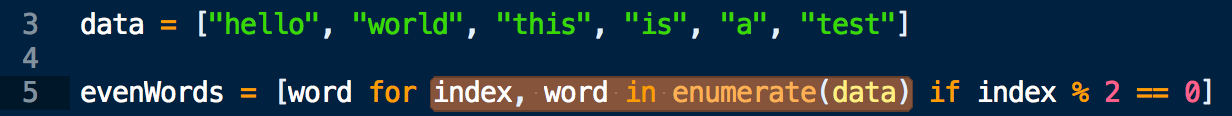
\includegraphics[width=0.95\columnwidth]{figures/highlight.png} 

\end{itemize}

Note that all these limitations of written tutorials are not specific to
Google Docs; related tools likely face similar issues.

\rev{Although we did not directly compare Torta to screencast videos for
this study, several creators mentioned the similarities between Torta
and screencast recording. For instance, S5 said, \emph{``This [Torta]
isn't any different from recording a screencast and I can also do
editing, annotation and validation."} And S2 mentioned, \emph{``I think I
would use this over recording a screencast despite the additional
processing time since the editor allows easier basic editing, like
dropping steps, which is easier than using a full video editor."}}

Subjects also conveyed perceived shortcomings of Torta's creation
workflow: It took some a while to get used to Torta segmenting videos
based on OS events such as GUI window switches, so they had to learn to
finish a full sentence of narration before switching in order to avoid
awkward audio cuts. They wanted to have more diverse format choices
than the step-by-step GUI-window-delimited structure that Torta imposes.
They also felt written tutorials were more flexible and less constraining,
though they take much more work to make.

Finally, \tab{tab:creator-study} shows that 9 out of 10 subjects created tutorials faster using Torta than
Google Docs.
For the five who used Torta first, they took around 1.1 times longer to
create the GDocs version (the harmonic mean of their time differences);
for the five who used GDocs first, they took an average of 2 times
longer in GDocs. This speed difference is likely due to them needing to spend
time planning out their tutorial's structure during their first attempt,
regardless of tool. \rev{This phenomenon likely resulted in a significant learning
effect since by the time they tried the second condition, they already
knew exactly what tutorial they wanted to create.} However, even when using
Torta first, subjects still
found it to be slightly faster. But we do not want to overemphasize these
timing numbers because the primary design goal of Torta was not to optimize
for tutorial creation speed.


\subsection{Tutorial Consumer \rev{Pilot Study}}

Although in the prior study we had creators self-assess the quality of their own Torta and
GDocs tutorials, we also wanted to get an assessment from the actual
target audience: students. Thus, we ran a \rev{follow-up pilot study} where students
followed the tutorials created by the TAs in the prior study and
compared their perceptions of Torta vs.\ GDocs from their perspectives
as tutorial consumers.


\emph{\textbf{Procedure}}: We recruited 6 undergraduate computer science
students each for a one-hour lab study. We had 3 subjects try to follow
a Torta-generated tutorial; then we showed them the Google Docs version
of the \emph{same} tutorial and had them compare and contrast the two
formats. We had the other 3 subjects try to follow a Google Docs
tutorial, and then had them compare it to its Torta counterpart. We did
not have each subject try to follow both tutorials since they would already
know how to perform the task after following the first one.

For this study, we picked the Node.js web programming tutorial created by
S2 since it was the most complex one. However, two subjects did
not have enough technical background to understand it, so instead we
gave them the singly-linked list tutorial created by S7 (one used
Torta, one used GDocs).


\emph{\textbf{Results}}: All 6 subjects successfully completed the
tutorial tasks in their given format. Both sets of 3 subjects (i.e.,
those who tried to follow the Torta tutorial then saw the Google Docs
version, and vice versa) preferred consuming Torta tutorials over Google
Docs for a variety of reasons, including:

%in \todo{15--18 minutes}; there were no major noticeable differences in
%completion times between Torta and Google Docs.


\begin{itemize}\itemsep0pt

\item \emph{Torta tutorials were better-structured}: Once subjects got
used to Torta's structure, they appreciated its predictability and could
skip over parts that did not interest them. In contrast, GDocs does not
impose any structure, so tutorials created within it felt more uneven in
pace. Subjects also commented that the consistency in Torta's format
would be good for a series of related tutorials across an entire course.

\item \emph{Torta tutorials more information-dense}: Most subjects
commented that Torta tutorials were more information-dense than GDocs
since they were narrated by voice and included automatically-traced
filesystem and command info. The GDocs versions could not include many
details due to lack of time for creators to write out everything
explicitly.

\item \emph{GUI apps better explained with mini-videos}: All subjects
felt that video was a much better way to demonstrate GUI applications
such as Postman rather than seeing a series of screenshots in GDocs.
They also appreciated each video being short and focused on only one
window.

\item \emph{Torta provides context behind file diffs}: When using GDocs
to create tutorials involving code, most creators ended up simply
pasting the new bits of code written in each step into the doc without
adequate surrounding context. Thus, subjects were confused about where
those pieces of code were supposed to be placed. In contrast, Torta
automatically generates file diffs and shows the original file contents
along with mini-videos to give students the proper context.

\item \emph{Torta's Validate and Run buttons were popular}: All
Torta-using subjects tried the Validate and Run buttons and commented that they seemed very
useful. They liked using Validate to avoid minor errors
compounding in later steps.

%\item \emph{Torta's collapsable steps were useful}: Several subjects
%used the collapse button next to steps and sub-steps to mark those
%parts as ``done" when they were following the tutorial so that they
%could keep track of their place.


\end{itemize}

However, one student (who had the most web dev experience) preferred
skimming a well-written GDocs tutorial rather than having to play the
Torta mini-videos and listen to audio narration at each step. Torta also
lets creators write HTML annotations for each step, but due to our user
study's short time limit, creators did not write much text in their
Torta tutorials.

\rev{Finally, although we did not directly compare Torta to
raw screencast videos for this study, several subjects
implicitly compared Torta with their prior experiences of watching
screencasts. For instance,
S11 said, \emph{``A lot of times when I'm watching coding videos on
YouTube, I wish I would have had a way to copy code and commands. This
[Torta] makes that way easier."}
%
S13 said: \emph{``I think cropping videos to the frontmost window is
great since it narrows focus to just that window. Many screencasts I
watch record the entire screen."}
%
S13 also mentioned: \emph{``I liked Torta breaking the video into steps.
On YouTube, video descriptions sometimes have links to different parts
of the video but using this [Torta] is much easier because I see the
parts of the video already split up."} }

